% ! TeX root = document.tex
\begin{frame}{Challenges}
  %% Background
  \only<1-4>{ 
    \begin{backgroundblock} 
      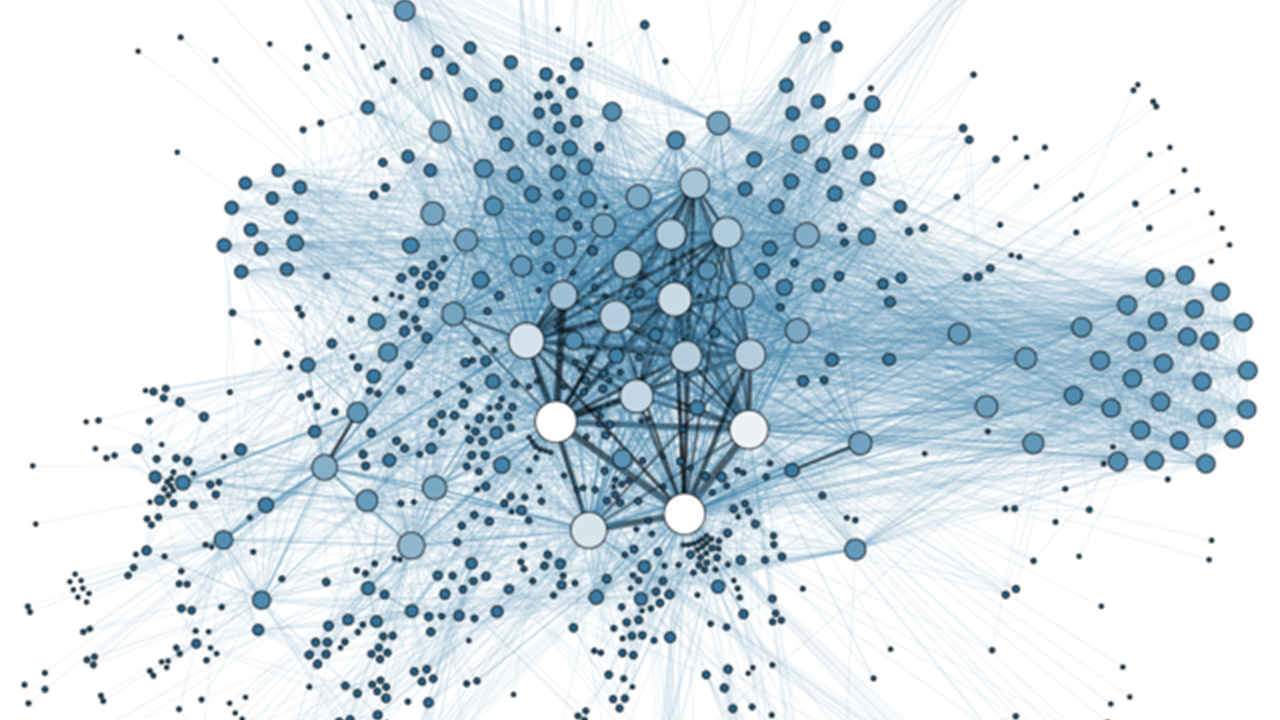
\includegraphics[width=\paperwidth]{img/complex-network.png} 
    \end{backgroundblock} 
  }
  \only<5-6>{ 
    \begin{backgroundblock} 
      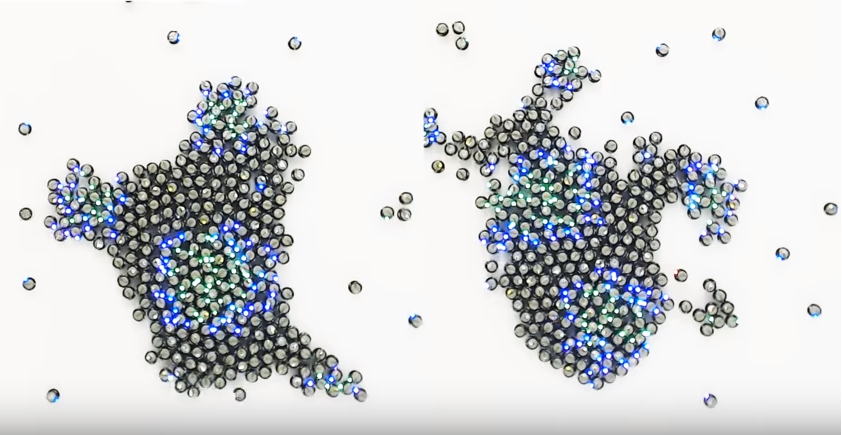
\includegraphics[height=\paperheight]{img/swarms.png}
    \end{backgroundblock} 
  }
  \begin{card}
    \begin{itemize}
      \item<1-| alert@1> Complex and layered networks
      \begin{itemize}
        \item <2-| alert@2>Large scale
        \item <3-| alert@3>Heterogenous
        \item <4-| alert@4>Dynamic
      \end{itemize}
      \item<5-| alert@5> Distributed control
      \item<6-| alert@6> Environmental changes
    \end{itemize}
  \end{card}
\end{frame}